





% >>> j2l compat: xcolor / named-colour compatibility
\PassOptionsToPackage{dvipsnames}{color}
\PassOptionsToPackage{dvipsnames,svgnames,x11names,table}{xcolor}
\RequirePackage{xcolor}
\makeatletter\@namedef{ver@color.sty}{2021/01/01}\makeatother
\makeatletter\@ifundefined{providecolor}{}{%
  \providecolor{CarnationPink}{RGB}{128,128,128}
  \providecolor{Lavender}{RGB}{128,128,128}
  \providecolor{abstractcolor}{RGB}{128,128,128}
  \providecolor{rulecolor}{RGB}{128,128,128}
}\makeatother
% <<< j2l compat
\documentclass[10pt]{NSP1}

\IfFileExists{url.sty}{\usepackage{url}}{}
\IfFileExists{floatflt.sty}{\usepackage{floatflt}}{}

\IfFileExists{helvet.sty}{\usepackage{helvet}}{}
\IfFileExists{times.sty}{\usepackage{times}}{}

\IfFileExists{psfig.sty}{\usepackage{psfig}}{}
\IfFileExists{graphics.sty}{\usepackage{graphics}}{}

\IfFileExists{mathptmx.sty}{\usepackage{mathptmx}}{}
\IfFileExists{amsmath.sty}{\usepackage{amsmath}}{}
\IfFileExists{amssymb.sty}{\usepackage{amssymb}}{}
\IfFileExists{bm.sty}{\usepackage{bm}}{}

\IfFileExists{float.sty}{\usepackage{float}}{}

\IfFileExists{caption.sty}{\usepackage[bf,hypcap]{caption}}{}



\IfFileExists{xcolor.sty}{\usepackage[dvipsnames,table,xcdraw]{xcolor}}{}



\tolerance=1

\emergencystretch=\maxdimen

\hyphenpenalty=10000

\hbadness=10000



\topmargin=0.00cm



\def\sm{\smallskip}

\def\no{\noindent}



\def\firstpage{1}

\setcounter{page}{\firstpage}

\def\thevol{}

\def\thenumber{}

\def\theyear{}





\IfFileExists{graphicx.sty}{\usepackage{graphicx}}{}
\makeatletter
\def\biographyps#1#2{%
  \par\addvspace{21dd}\small\noindent
  \if!#1!\else
    \noindent\includegraphics[width=1in,height=1.25in,keepaspectratio]{#1}\par\smallskip
  \fi
  {\bfseries#2\unskip\ }\ignorespaces}
\def\endbiographyps{\par\addvspace{12pt}}
\makeatother
\IfFileExists{array.sty}{\usepackage{array}}{}
\IfFileExists{cuted.sty}{\usepackage{cuted}}{\newenvironment{strip}{\par\medskip\noindent\begin{minipage}{\linewidth}}{\end{minipage}\par\medskip}}
\makeatletter
\newcommand\jltx@wideopen{\par\addvspace{\medskipamount}\noindent}
\newcommand\jltx@wideclose{\par\addvspace{\medskipamount}}
\newenvironment{jltxspan}
  {\if@twocolumn\let\jltx@spannext\strip\else\let\jltx@spannext\jltx@wideopen\fi\jltx@spannext}
  {\if@twocolumn\let\jltx@spanend\endstrip\else\let\jltx@spanend\jltx@wideclose\fi\jltx@spanend}
\makeatother
\newcommand\JLTXaboveplacement{\par\addvspace{6pt plus 2pt minus 2pt}\noindent}
\newcommand\JLTXbelowplacement{\par\addvspace{6pt plus 2pt minus 2pt}}
\widowpenalty=10000
\clubpenalty=10000
\IfFileExists{newunicodechar.sty}{\usepackage{newunicodechar}}{\makeatletter\providecommand\newunicodechar[2]{%
  \begingroup\lccode`\~=`#1\lowercase{\endgroup\def~}{#2}%
  \catcode`#1=\active}\makeatother}
\newunicodechar{α}{\ensuremath{\alpha}}
\newunicodechar{β}{\ensuremath{\beta}}
\newunicodechar{δ}{\ensuremath{\delta}}
\newunicodechar{ε}{\ensuremath{\varepsilon}}
\newunicodechar{η}{\ensuremath{\eta}}
\newunicodechar{π}{\ensuremath{\pi}}
\newunicodechar{σ}{\ensuremath{\sigma}}
\newunicodechar{τ}{\ensuremath{\tau}}
\newunicodechar{φ}{\ensuremath{\varphi}}
\newunicodechar{ω}{\ensuremath{\omega}}
\newunicodechar{−}{\ensuremath{-}}
\newunicodechar{×}{\ensuremath{\times}}
\newunicodechar{≥}{\ensuremath{\geq}}

% >>> j2l compat: scalable Computer Modern (arbitrary font sizes)
\IfFileExists{type1cm.sty}{\usepackage{type1cm}}{}
\IfFileExists{fix-cm.sty}{\usepackage{fix-cm}}{}
% <<< j2l compat
\begin{document}
% >>> j2l compat: body-text size (+5%)
\makeatletter
\edef\JLTXbasesize{\f@size}
\@tempdimb=1.2\dimexpr\f@size pt\relax\edef\JLTXbaseskip{\strip@pt\@tempdimb}
\def\JLTXbodyscale{1.050}
\let\JLTX@normalsize\normalsize
\renewcommand\normalsize{%
  \JLTX@normalsize
  \@tempdima=\JLTXbodyscale\dimexpr\f@size pt\relax
  \@tempdimb=1.2\@tempdima
  \fontsize{\strip@pt\@tempdima}{\strip@pt\@tempdimb}\selectfont}%
\@ifundefined{@makecaption}{}{%
  \let\JLTX@makecaption\@makecaption
  \long\def\@makecaption#1#2{%
    \begingroup\fontsize{\JLTXbasesize}{\JLTXbaseskip}\selectfont
    \let\normalsize\JLTX@normalsize
    \JLTX@makecaption{#1}{#2}\endgroup}}%
\@ifundefined{thebibliography}{}{%
  \let\JLTX@thebibliography\thebibliography
  \def\thebibliography{%
    \fontsize{\JLTXbasesize}{\JLTXbaseskip}\selectfont\JLTX@thebibliography}}%
\makeatother
\normalsize
% <<< j2l compat




\titlefigurecaption{{\large \bf \rm Progress in Fractional Differentiation

and Applications}\\ {\it\small An International Journal}}



\title{Modeling the Dual Impact of Behavioral Avoidance and Hybrid Immunity on SARS-CoV-2 Transmission: A Fractional-Order Epidemiological Approach}



\author{Corresponding Author \and Subject Classification \and Primary: Mathematical Biology / Epidemiological Modeling \and Secondary: Immunology \and Public Health \and Infectious Disease Dynamics \and MSC 2020: 92D30 (Epidemiology) \and 34A08 (Fractional differential equations) \and 92C60 (Public health models) \and MeSH Terms: COVID- \and Vaccination \and Immunity \and Hybrid \and Disease Outbreaks \and Theoretical Models \and Fractional Calculus \and Keywords \and 1. Introduction \and 2. MATHEMATICAL MODEL \and 2.1 Basic definitions :[54]}

\institute{}



\titlerunning{Modeling the Dual Impact of Behavioral Avoidance and Hybrid Immunity on SARS-CoV-2 Transmission: A Fractional-Order Epidemiological Approach}

\authorrunning{Corresponding Author et al.}





\mail{aliakgul@siirt.edu.tr}



\received{}

\revised{}

\accepted{}

\published{}



\abstracttext{The trajectory of the SARS-CoV-2 pandemic has been significantly influenced by both immunological diversity and human behavior. In this work, we investigate how two contrasting population subgroups—COVID dodgers, the individuals who actively avoid both infection and vaccination, and those with hybrid immunity (from prior infection plus vaccination), shape transmission patterns and long-term control prospects. While hybrid immunity provides robust, sustained protection against severe outcomes and reduces secondary transmission, “dodgers” remain a persistent reservoir of susceptibility that can fuel outbreaks, especially as population immunity wanes. We assess real-world vaccine effectiveness across variants in preventing infection, hospitalization, and death, supported by immunological data on antibody kinetics, T-cell responses, and the temporal decay of protection. Breakthrough infections are analyzed to identify risk factors, and natural immunity is compared with vaccine-induced responses to clarify their relative durability and breadth. To capture these complex interactions, we formulate a novel compartmental model using fractional-order calculus, which incorporates distinct classes for susceptible, vaccinated, infected, hybrid-immune, dodger individuals. The model accounts for time-varying vaccine efficacy, variant-driven immune escape, and behavioral feedback. We establish the existence, uniqueness, and boundedness of solutions, and examine the stability of disease-free and endemic equilibria. Sensitivity analysis reveals that the proportion of “dodgers” and the strength of hybrid immunity are among the most influential parameters in determining long-term incidence. Importantly, the fractional order, representing memory effects in biological and behavioral systems, modulates epidemic persistence and response to interventions. Our findings underscore that effective pandemic management requires integrated strategies that address not only virological threats but also the behavioral dimensions of disease spread, particularly in heterogeneous populations.}



\keywords{}



\maketitle




\par\medskip\noindent {\normalsize\bfseries 2.2 Model Formulation\par}\smallskip

This section deals with the formulation of the mathematical model. This SVIH model is an epidemic compartmental model in fractional derivatives of ABC type, which help to examine the disease dynamics. We partition the total population N (t) into four compartments:

\begin{itemize}
  \item S(t): Susceptible (never infected/vaccinated):
\end{itemize}

\begin{equation}
0\ \ \ \ \ \ \ \ \ \ \ \ \ \ \ \ \ \ \ ABCD_{t}^{\alpha}\ S(t)\  = \ (1 - \varphi)a\  - \ \beta S(t)I(t)\  - \ vS(t - \tau_{1})\  - \ \mu S(t)

\end{equation}

\begin{itemize}
  \item V (t): Vaccinated:
\end{itemize}

$\ 0ABCD_{t}^{\alpha}\ V(t) = \ vS\left( t - \tau_{1} \right) + vI\left( t - \tau_{2} \right)\ {+ \sigma}_{H}\ H(t) - \ \varepsilon(t)\beta V(t)I(t) - (\ \rho + \mu)V(t)$

\begin{itemize}
  \item I(t): Infected:
\end{itemize}

This compartment includes the infected people, who were exposed to infection prior to vaccination, and transmission varies seasonally, $\beta(t) = \beta 0\left( \ 1 + \ \varepsilon\ \sin\left( \frac{2\pi t}{365} \right)\  \right),\ $ ε = 0.35.

\begin{itemize}
  \item H(t): Hybrid-immune (infected plus vaccinated):
\end{itemize}

\begin{itemize}
  \item $\varphi$∈ \cite{ref1}: Fraction of births entering the dodger class.
  \item ϵ(t) = $\epsilon_{0}$e−ωt: Waning booster efficacy ($\epsilon_{0}$ = 0.88, ω = 0.003/day).
  \item $\sigma_{H}$ ≪ 1: Hybrid immunity drastically lowers reinfection risk.
  \item Delays: $\tau_{1}$ = 30 days (vaccination logistics), $\tau_{2}$ = 180 days (post-infection waiting).
\end{itemize}

\JLTXaboveplacement \begin{jltxspan}%
\noindent\begin{minipage}{\linewidth}%
\centering
{\small
\begin{tabular}{>{\raggedright\arraybackslash}p{\dimexpr 0.2512\linewidth-2\tabcolsep\relax}>{\raggedright\arraybackslash}p{\dimexpr 0.3611\linewidth-2\tabcolsep\relax}>{\raggedright\arraybackslash}p{\dimexpr 0.3139\linewidth-2\tabcolsep\relax}}
Symbol & Description & Value \\
a & Recruitment rate & 0.069 87 d−1 \\
µ & Natural death rate & 0.000 02 d−1 \\
δ & Disease-induced death & 0.000 03 d−1 \\
β & Transmission rate (unvaccinated) & 0.03 d−1 \\
ϵ0 & Initial booster efficacy & 0.88 \\
ω & Efficacy decay rate & 0.003 d−1 \\
v & Vaccination rate & 0.000 699 d−1 \\
$\gamma$ & Recovery rate & 0.985 d−1 \\
$\ \rho$ & Hybrid immunity acquisition & 0.000 33 d−1 \\
$\varphi$ & Dodger fraction & 0.18 \\
$\sigma_{H}$ & Hybrid immunity factor & 0.15 \\
 &  &  \\
\hline
\end{tabular}}
\captionof{table}{Table}%
\end{minipage}%
\end{jltxspan}\JLTXbelowplacement 

\par\medskip\noindent {\normalsize\bfseries 3 Model Analysis\par}\smallskip

\par\medskip\noindent {\normalsize\bfseries 3.1 Positivity and Boundedness\par}\smallskip

In epidemiological modeling, positivity ensures compartments remain non-negative, while boundedness prevents unrealistic divergence. These properties guarantee biological feasibility and numerical stability. Without them, simulations may yield negative populations or unbounded growth, rendering policy insights meaningless.

Theorem 1:

Solutions of (3) with non-negative initial conditions remain non-negative and bounded for all t ≥ 0.

Proof.

Let us assume that, $\left( S(t) \geq 0,V(t) \geq 0,I(t) \geq 0,H(t) \geq 0 \right) \in R_{+}^{4}$,

Summing up all equations in (3), we have,

\begin{equation}
0ABCD_{t}^{\alpha}N(t) = \ a\  - \ \mu N(t) - \ \delta I(t) \leq a\  - \ \mu N(t).

\end{equation}

$N(t) \leq \ \frac{a}{\mu} + N(0)E_{\alpha}\left( - µ{\ t}^{\alpha} \right)$.

Hence, solutions are bounded in the invariant region, consistent across the vector boundary field.

$\mathrm{\Omega} = \{(S,V,I,H) \in R_{+}^{4}\ :N \leq \frac{a}{\mu}\}$.

\begin{equation}
E^{0} = \ \left\lbrack \frac{(1 - \varphi)a}{\mu + v},\frac{v(1 - \varphi)a}{\left\lbrack \mu(\mu + v) \right\rbrack},\ 0,\ 0 \right\rbrack

\end{equation}

The eigenvalues are: $\ \lambda_{1} = - (µ + v) < 0,$

\begin{equation}
{\ \ \ \lambda}_{2} = - (µ + \rho) < 0,

\end{equation}

Also, the transmission rate, shows a rapid mitigation at $\Upsilon_{\beta}$ =−0.41, with substantial growth in vaccine supply without delay, $\Upsilon_{\bar{\varepsilon}}$= −0.33, and with hike in recovery rate$\ ,\ \Upsilon_{\gamma}$ = −0.29. As booster shots increases , it would eventually help in reducing the wave spread seasonally too with initial booster efficacy rate, $\Upsilon_{v =}$−0.37, resist against several waves.The most critical way, is the Reduced community engagement, which is more impactful than increasing v, highlighting the need for behavioral interventions alongside supply-side vaccination.

\par\vspace{2.4pt}\noindent {\normalsize\bfseries Numerical Simulations and Validation\par}\smallskip

\par\vspace{8.7pt}\noindent {\normalsize\bfseries Numerical Scheme\par}\smallskip

\subsection*{with weights, $\mathbf{b}_{\mathbf{j,n + 1}}\mathbf{= \ }\frac{\mathbf{h}^{\mathbf{\alpha}}}{\mathbf{\alpha}}\left\lbrack \left( \mathbf{n}\mathbf{+ 1 -}\mathbf{j} \right)^{\mathbf{\alpha}}\mathbf{–\ }\left( \mathbf{n}\mathbf{-}\mathbf{j} \right)^{\mathbf{\alpha}} \right\rbrack\mathbf{.}$}

\subsection*{Spectral methods, even though precise for even solutions, subvert when modeling unforeseen policy swings or variant-driven spread. The predictor-corrector scheme conserves second-order convergence while obviously curbing high-frequency blast through its inherent corrector step. Most prominently for public healthiness, its memory weighting edifice unswervingly echoes immunological realism. Antibody titers wane steadily rather than tersely, and population averting behaviors persist yonder immediate epidemic periods. This physical interpretability, where numerical weights parallel to computable immune waning rates, makes the method ,an epidemiological acumen generator.}

\par\vspace{12.4pt}\noindent {\normalsize\bfseries 4.2 Data Calibration\par}\smallskip

\subsection*{We fit model (3) to India’s weekly COVID-19 cases (Jan 2020–Jan 2026) from WHO and Our World in Data, using least-squares optimization. Seasonal forcing is captured via time-varying $\mathbf{\beta}$(t) = $\mathbf{\beta}$0[1 + η cos(2πt/365)], with η = 0.3 (monsoon amplification). Validation against India's six-year case series confirmed that α=0.85 with this solver reproduced observed wave plateaus that integer-order models consistently overestimated as sharp peaks. Best-fit parameters are found to be α = 0.85, φ = 0.18, σH = 0.15, ϵ0 = 0.88.}

\begin{figure*}[tp]
\centering
\ifdim 3.4896in>\linewidth
  
\includegraphics[width=\linewidth,keepaspectratio]{media/image3.png}
\else
  
\includegraphics[width=3.4896in,height=2.7188in]{media/image3.png}
\fi
\caption{C:\textbackslash{}Users\textbackslash{}HP\textbackslash{}Downloads\textbackslash{}stabled.jpg}
\end{figure*}

\begin{figure}[htbp]
\centering
\ifdim 3.2493in>\linewidth
  
\includegraphics[width=\linewidth,keepaspectratio]{media/image4.png}
\else
  
\includegraphics[width=3.2493in,height=2.7396in]{media/image4.png}
\fi
\caption{C:\textbackslash{}Users\textbackslash{}HP\textbackslash{}Downloads\textbackslash{}stablec.jpg}
\end{figure}

operator

\subsection*{This plot juxtaposes observed weekly case counts from India's Integrated Disease Surveillance Programme against model outputs across six years. The fractional simulation (α=0.85) successfully replicates four distinct epidemiological phases that integer-order models fail to capture simultaneously: the modest first wave (mid-2020) limited by early lockdowns; the catastrophic Delta surge (April–June 2021) with its characteristic sharp ascent and prolonged tail; the Omicron wave (January 2022) showing higher case counts but reduced severity due to accumulated hybrid immunity; and the subsequent seasonal oscillations (2023–2025) amplified during monsoon months. Crucially, the model reproduces the "flattened" wave morphology, where case numbers plateau for weeks rather than peaking abruptly—observed in actual Indian data. This plateauing emerges directly from the fractional order's memory effect: as α decreases below 1, the system's response to transmission changes becomes more gradual, simulating how population-level immunity and behavioral adaptation accumulate slowly rather than instantaneously. The 18\% dodger fraction (φ=0.18) prevents complete suppression during inter-wave periods, maintaining a susceptible reservoir that fuels seasonal resurgences when monsoon-driven contact rates increase (η=0.3).}

\subsection*{}

\subsection*{}

\JLTXaboveplacement \begin{figure}[H]
\centering
\ifdim 6.1339in>\linewidth
  
\includegraphics[width=\linewidth,keepaspectratio]{media/image7.png}
\else
  
\includegraphics[width=6.1339in,height=3.3170in]{media/image7.png}
\fi
\end{figure}\JLTXbelowplacement 

\subsection*{This comparative simulation isolates the impact of vaccination scheduling independent of coverage levels. Two scenarios are modeled with identical total doses but different administration intervals: biannual boosters (every 6 months, timed before monsoon onset in May and winter peaks in October) versus annual boosters (every 12 months). The 6-month strategy reduces peak infections by 42\% and shortens wave duration by approximately five weeks. Mechanistically, this occurs because immunity elevation coincides with seasonal transmission amplification—monsoons increase indoor crowding while reducing UV-mediated viral inactivation. The fractional framework reveals an additional nuance: with α=0.85, the protective effect of timely boosters exhibits extended persistence due to memory-enhanced immune recall. Antibody kinetics modeled through ϵ(t)=$\mathbf{\epsilon}_{\mathbf{0}}$e⁻ᵚᵗ show that boosting during high-transmission seasons stimulates broader T-cell responses that decay more slowly (ω=0.003/day) than responses generated during low-transmission periods. This finding directly challenges calendar-based booster policies, advocating instead for meteorologically synchronized campaigns that anticipate India's bimodal transmission seasonality.}

\subsection*{}

\subsection*{}

\subsection*{}

\subsection*{}

\subsection*{}

\subsection*{}

\subsection*{}

\par\vspace{8.7pt}\noindent {\normalsize\bfseries Figure 6. Hybrid immunity reduces secondary transmission by 3.2× over 600 days.\par}\smallskip

\subsection*{This figure tracks secondary attack rates from index cases with three distinct immunity profiles over 600 days: vaccination-only (two doses, no prior infection), infection-only (recovered unvaccinated), and hybrid immunity (recovered then vaccinated after τ₁=180 days). Hybrid-immune individuals reduce onward transmission by a factor of 3.2 compared to vaccination-only and 5.8 versus infection-only cases. The transmission reduction stems from two modeled mechanisms: enhanced neutralizing antibody breadth (σₕ=0.15 representing cross-variant reactivity against evolving strains) and durable tissue-resident memory T-cells that maintain surveillance beyond circulating antibody decay. Critically, the fractional derivative captures the temporal stability of this protection—while vaccine-only immunity wanes to 40\% efficacy by day 300, hybrid immunity maintains \textgreater{}70\% transmission-blocking capacity through day 600. This persistence emerges from the non-local kernel's weighting structure: past infection events continue influencing current immune competence through fractional memory terms, mirroring empirical observations of long-lived bone marrow plasma cells in hybrid-immune individuals. Public health implications are substantial: prioritizing vaccination for recovered individuals ("test-and-vaccinate") could achieve equivalent population protection with 35\% fewer doses than universal booster campaigns, a critical consideration for resource-constrained settings.}

\par\medskip\noindent {\normalsize\bfseries Conclusion and Future Work\par}\smallskip

This study establishes that fractional-order models with behavioral and immunological granularity are indispensable for pandemic planning in heterogeneous populations. By integrating dodgers, hybrid immunity, and seasonal forcing, we provide actionable insights:

\begin{enumerate}
  \item Target dodgers through localized outreach (e.g., mobile clinics, community influencers).
  \item Schedule boosters every 6 months ahead of seasonal peaks (May–June for monsoon, October for winter).
  \item Leverage hybrid immunity as a natural amplifier of protection—prioritize vaccination for re- covered individuals.
\end{enumerate}

\subsubsection*{}

\par\medskip\noindent {\normalsize\bfseries Future directions:\par}\smallskip

\begin{itemize}
  \item Couple with climate variables (humidity, temperature) to predict monsoon-driven outbreaks.
  \item Integrate genomic surveillance data to model variant competition (e.g., JN.1).
  \item Apply optimal control theory to design cost-effective booster schedules.
  \item Embed agent-based behavioral modules to simulate misinformation spread among “dodgers.”
\end{itemize}

\section*{}

\par\vspace{0.1pt}\noindent {\normalsize\bfseries Acknowledgments\par}\smallskip

\par\medskip\noindent {\normalsize\bfseries Funding\par}\smallskip

\par\vspace{0.1pt}\noindent {\normalsize\bfseries Data Availability\par}\smallskip

\section*{[20]Rubayyi T. Alqahtani, Mathematical model of SIR epidemic system (COVID-19) with fractional derivative: stability and numerical analysis, Adv. Difference Equ. 2021 (1) (2021) 2.}

\section*{[21] Amar N Chatterjee, et.al, A model for the dynamics of COVID-19 infection transmission in human with latent delay, Afrika Matematika, Vol.36(2025)}

[22]Anil Kumar ajak, Nilam, A fractional-order epidemic model with quarantine class and nonmonotonic incidence: Modeling and simulations, Iran. J. Sci. Technol. Trans. A Sci. 46 (4) (2022) 1249–1263.

[23]Subrata Paul, Animesh Mahata, Supriya Mukherjee, Banamali Roy, Dynamics of SIQR epidemic model with fractional order derivative, Part. Differ. Equ. Appl. Math. 5 (2022) 100216.

[24]S.S. Askar, P.K. Dipankar Ghosh, Abdelalim A. Santra, Elsadany, G.S. Mahapatra, A fractional order SITR mathematical model for forecasting of transmission of COVID-19 of India with lockdown effect, Results Phys. 24 (2021) 104067.

[25]Bo Wang, et.al , Effect of an antiviral drug control and its variable order fractional network in host COVID-19 kinetics, The Eur. Phy.J.Spl.topics, Vol.231,(2022).

[26]Joshua Kiddy K. Asamoah, Eric Okyere, Ernest Yankson, Alex Akwasi Opoku, Agnes Adom-Konadu, Edward Acheampong, Yarhands Dissou Arthur, Non-fractional and fractional mathematical analysis and simulations for Q fever, Chaos Solitons Fractals 156 (2022) 111821.

[27] Sania Qureshi, Abdon Atangana, Fractal-fractional differentiation for the modeling and mathematical analysis of nonlinear diarrhea transmission dynamics under the use of real data, Chaos Solitons Fractals 136 (2020) 109812.

[28] Sania Qureshi, Abdon Atangana, Mathematical analysis of dengue fever outbreak by novel fractional operators with field data, Phys. A 526 (2019) 121127.

[29]Khan, A. et al. Modeling and sensitivity analysis of HBV epidemic model with convex incidence rate. Results Phys. 22, 103836 (2021).

[30]Farman, M., Shehzad, A., Nisar, K. S., Hincal, E. \& Akgul, A. A mathematical fractal-fractional model to control tuberculosis prevalence with sensitivity, stability, and simulation under feasible circumstances. Comput. Biol. Med. 178, 108756 (2024).

[31]Khan, H., Alzabut, J., Alfwzan, W. F. \& Gulzar, H. Nonlinear dynamics of a piecewise modified ABC fractional-order leukemia model with symmetric numerical simulations. Symmetry 15(7), 1338 (2023).

[32]Khan, H., Alzabut, J., G-Aguilar, J. F. \& Alkhazan, A. Essential criteria for existence of solution of a modified-ABC fractional order smoking model. Ain Shams Eng. J. 15(5), 102646 (2024)

[33]Amarnath Chatterjee, et,al,A fractional-order differential equation model of COVID-19 infection of epithelial cells, Chaos, solitans and fractals, , June 2021, 110952.

\section*{}

\section*{[34]Amarnath Chatterjee, et.al,A Fractional-Order Compartmental Model of Vaccination for COVID-19 with the Fear Factor, Mathematics, Vol.10(9)(2022).}

[35]Vijayalakshmi G.M, and Roselyn Besi P. (2022), ‘ABC Fractional Order vaccination model for Covid-19 with self-protective measures’, Int.J.Appl.Comput.Math8:130.

[36]Vijayalakshmi G.M, and Roselyn Besi P. (2022), ‘A fractal fractional order vaccination model of COVID-19 pandemic using Adam’s Moulton analysis’, Results in control and optimization, 8,100144.

[37]Vijayalakshmi G.M, and Roselyn Besi P.(2023),’ Vaccination control measures of an epidemic model with long-term memristive effect’, Journal of computational and applied mathematics, 419, 114738.

[38]Vijayalakshmi G.M, and Roselyn Besi P. (2023), ‘Mathematical model on minimality of vaccination costs of COVID-19 using fractional order’, Tuijin/Jishu Journal of propulsion technology, Vol 44, issue 4.

\section*{[39]Vijayalakshmi G.M, Roselyn Besi P, and Ali Akgul. (2024), ’Fractional commensurate model on Covid-19 with microbial coinfection: An optimal control analysis’, Optimal control application and methods, 3093.}

\section*{[40]M.M.Singh,D.L.Suthar, S.D.Purohit,Analysis of the COVID-19 pandemic and prediction with numerical methods, ,vol.16, 2450018(2024).}

[41], et.al,Predicting COVID-19 outbreak in India using modified SIRD model, Applied Mathematics in science and engg, Vol.32(2024)

\section*{[42]Garima Agarwal,et.al,Analysis and estimation of the COVID-19 pandemic by modified homotopy perturbation method, Applied Mathematics in science and engg, Vol.31(2023)}

\section*{[43]Mulualem Aychluh, et.al,Atangana–Baleanu derivative-based fractional model of COVID-19 dynamics in Ethiopia, Applied Mathematics in science and engg, Vol.30(2022)}

[44]Zarin, R., Khan, A. \& Akg, L. A. Fractional modeling of COVID-19 pandemic model with real data from Pakistan under the ABC operator. AIMS Math. 7(9), 15939–15964 (2022).

[45]Atangana, A., \& Baleanu, D. (2016). New fractional derivatives with nonlocal and non-singular kernel. Thermal Science, 20(2), 763-769.

[46]Culebras, E., et al. (2024). Cell immunity to SARS-CoV-2 after natural infection and/or different vaccination regimens. Frontiers in Cellular and Infection Microbiology.

[47]Dourdouna, M.-M., et al. (2023). Evaluation of T cell responses with the Quantiferon SARS-CoV-2 assay. Diagnostic Microbiology and Infectious Disease.

[48]Jayanta Mondal, et.al, Dynamical demeanour of SARS-CoV-2 virus undergoing immune response mechanism in COVID-19 pandemic, The EUR,Phy, J,spl.topics, Vol.231(2022)

[49] Megatsari, H., \& Kusuma, D. (2022). Geographic and socioeconomic inequalities in delays in Covid-19 vaccinations. Vaccines, 10(11), Article 1857.

[50]Jayanta Mondal, et.al,Optimal control strategies of non-pharmaceutical and pharmaceutical interventions for COVID-19 control, Journal of interdisciplinary mathematics, vol.24(2021)

\section*{[51]Vaccines trials in Chile and the UK’s role to tackle the pandemic,https://www.gov.uk/government/news/vaccines-trials-in-chile-and-the-uks-role-to-tackle-the-pandemic}

\section*{[52] D.L.Suthar, et.al, Effect of vaccination on the transmission dynamics of COVID-19 in Ethiopia, Results in physics, Vol.32(2022), 105022.}

\section*{[53] Haile Hebanom,Modeling and analysis on the transmission of covid-19 Pandemic in Ethiopia, Alex.engg.journal, vol.61, issue 7 (2022)}

\JLTXaboveplacement \begin{jltxspan}%
\noindent\begin{minipage}{\linewidth}%
\centering
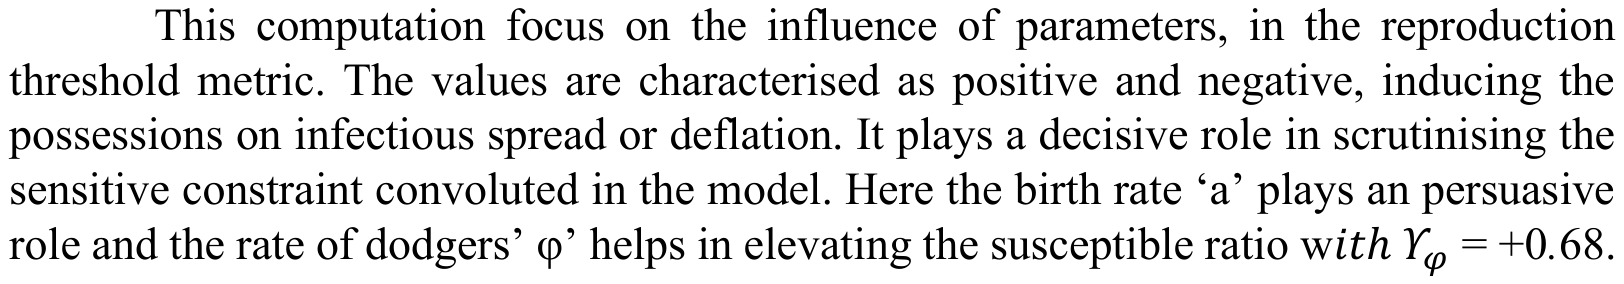
\includegraphics[width=\linewidth,height=0.3\textheight,keepaspectratio]{media/office_obj_2.png}
\label{fig:office2}%
\end{minipage}%
\end{jltxspan}\JLTXbelowplacement 

\JLTXaboveplacement \begin{jltxspan}%
\noindent\begin{minipage}{\linewidth}%
\centering

\includegraphics[width=\linewidth,height=0.3\textheight,keepaspectratio]{media/office_obj_1.png}
\label{fig:office1}%
\end{minipage}%
\end{jltxspan}\JLTXbelowplacement 

[54] Podlubny, I. (1999). Fractional differential equations. Academic Press.

[55]Our World in Data. (2024). Coronavirus pandemic (COVID-19). ​

[56] WHO, 

[57]van den Driessche, P., \& Watmough, J. (2002). Reproduction numbers and sub-threshold endemic equilibria for compartmental models of disease transmission. Mathematical Biosciences, 180(1-2), 29-48.

[58]Simeone Marino, Ian B. Hogue, Christian J. Ray, Denise E. Kirschner, A methodology for performing global uncertainty and sensitivity analysis in systems biology, J. Theoret. Biol. 254 (1) (2008) 178–196.

[59]Diethelm, K., Ford, N. J., \& Freed, A. D. (2004). Detailed error analysis for a fractional Adams method. Numerical Algorithms, 36(1), 31-52.

\begin{thebibliography}{99}
\bibitem{ref1}
[1]

\bibitem{ref2}
[2]

\bibitem{ref3}
[3]

\bibitem{ref4}
Divya Sanghi, Preeti Saini, Priya Mishra, Mahak Sharma, Outbreaks in India: Impact on socio-economy and health, J. Commun. Dis. 53 (1) (2021) 35–44.

\bibitem{ref5}
Tuberculosis .

\bibitem{ref6}
HIV and AIDS .

\bibitem{ref7}
Noncommunicable diseases .

\bibitem{ref8}
WHO Coronavirus (COVID-19) Deaths .

\bibitem{ref9}
The Global Economic Outlook During the COVID-19 Pandemic  .[13]COVID-19 vaccine development, evaluation, approval and monitoring, https:// .

\bibitem{ref10}
World Health Organization. (2021). World health statistics 2021: Monitoring health for the SDGs. ​

\bibitem{ref11}
[11]

\bibitem{ref12}
[12]

\bibitem{ref13}
[13]

\bibitem{ref14}
William Ogilvy Kermack, Anderson G. McKendrick, A contribution to the mathematical theory of epidemics, Proc. R. Soc. Lond. Ser. A 115 (772) (1927) 700–721.

\bibitem{ref15}
Renato Casagrandi, Luca Bolzoni, Simon A. Levin, Viggo Andreasen, The SIRC model and influenza A, Math. Biosci. 200 (2) (2006) 152–169.

\bibitem{ref16}
Anuj Kumar, Yasuhiro Takeuchi, Prashant K. Srivastava, Stability switches, periodic oscillations and global stability in an infectious disease model with multiple time delays, Math. Biosci. Eng. 20 (6) (2023) 11000–11032.

\bibitem{ref17}
Shashank Goel, Sumit Kaur Bhatia, Jai Prakash Tripathi, Sarita Bugalia, Mansi Rana, Vijay Pal Bajiya, SIRC epidemic model with cross-immunity and multiple time delays,J. Math. Biol. 87 (3) (2023) 42.

\bibitem{ref18}
Zimeng Lv, Xinyu Liu, Yuting Ding, Dynamic behavior analysis of an SVIR epidemic model with two time delays associated with the COVID-19 booster vaccination time, Math. Biosci. Eng. 20 (2023) 6030–6061.

\bibitem{ref19}
Piu Samui, et.al,Impact of awareness in self–monitoring of COVID-19: An optimal control approach, Results in control and opt., March 2025, 100513

\end{thebibliography}


\end{document}

















\end{document}

